% PODPISAC WYKRESY, 

\documentclass[12pt, a4paper]{article}\usepackage[]{graphicx}\usepackage[]{color}
%% maxwidth is the original width if it is less than linewidth
%% otherwise use linewidth (to make sure the graphics do not exceed the margin)
\makeatletter
\def\maxwidth{ %
  \ifdim\Gin@nat@width>\linewidth
    \linewidth
  \else
    \Gin@nat@width
  \fi
}
\makeatother

\definecolor{fgcolor}{rgb}{0.345, 0.345, 0.345}
\newcommand{\hlnum}[1]{\textcolor[rgb]{0.686,0.059,0.569}{#1}}%
\newcommand{\hlstr}[1]{\textcolor[rgb]{0.192,0.494,0.8}{#1}}%
\newcommand{\hlcom}[1]{\textcolor[rgb]{0.678,0.584,0.686}{\textit{#1}}}%
\newcommand{\hlopt}[1]{\textcolor[rgb]{0,0,0}{#1}}%
\newcommand{\hlstd}[1]{\textcolor[rgb]{0.345,0.345,0.345}{#1}}%
\newcommand{\hlkwa}[1]{\textcolor[rgb]{0.161,0.373,0.58}{\textbf{#1}}}%
\newcommand{\hlkwb}[1]{\textcolor[rgb]{0.69,0.353,0.396}{#1}}%
\newcommand{\hlkwc}[1]{\textcolor[rgb]{0.333,0.667,0.333}{#1}}%
\newcommand{\hlkwd}[1]{\textcolor[rgb]{0.737,0.353,0.396}{\textbf{#1}}}%
\let\hlipl\hlkwb

\usepackage{framed}
\makeatletter
\newenvironment{kframe}{%
 \def\at@end@of@kframe{}%
 \ifinner\ifhmode%
  \def\at@end@of@kframe{\end{minipage}}%
  \begin{minipage}{\columnwidth}%
 \fi\fi%
 \def\FrameCommand##1{\hskip\@totalleftmargin \hskip-\fboxsep
 \colorbox{shadecolor}{##1}\hskip-\fboxsep
     % There is no \\@totalrightmargin, so:
     \hskip-\linewidth \hskip-\@totalleftmargin \hskip\columnwidth}%
 \MakeFramed {\advance\hsize-\width
   \@totalleftmargin\z@ \linewidth\hsize
   \@setminipage}}%
 {\par\unskip\endMakeFramed%
 \at@end@of@kframe}
\makeatother

\definecolor{shadecolor}{rgb}{.97, .97, .97}
\definecolor{messagecolor}{rgb}{0, 0, 0}
\definecolor{warningcolor}{rgb}{1, 0, 1}
\definecolor{errorcolor}{rgb}{1, 0, 0}
\newenvironment{knitrout}{}{} % an empty environment to be redefined in TeX

\usepackage{alltt}

%%%%%%%%%%%%%%%%%%%%%%%%%%%%%%%%%%%%%%%%%%%%%%%%%%%%%%%%%%%%%%%%
% LaTeX packages
%\usepackage[OT4]{polski}
\usepackage[utf8]{inputenc}
\usepackage[top=2.5cm, bottom=2.5cm, left=2cm, right=2cm]{geometry}
\usepackage{graphicx}
\usepackage{amsmath}
\usepackage{float}
\usepackage[colorlinks=true, linkcolor=blue]{hyperref}


%%%%%%%%%%%%%%%%%%%%%%%%%%%%%%%%%%%%%%%%%%%%%%%%%%%%%%%%%%%%%%%%
% global settings


\IfFileExists{upquote.sty}{\usepackage{upquote}}{}
\begin{document}

%%%%%%%%%%%%%%%%%%%%%%%%%%%%%%%%%%%%%%%%%%%%%%%%%%%%%%%%%%%%%%%%
% title page
\title{Estimation theory -- Laboratory 1.}
\author{Agnieszka Szkutek, 208619 \\ Marta Frankowska, 208581}
\maketitle
\tableofcontents 


%%%%%%%%%%%%%%%%%%%%%%%%%%%%%%%%%%%%%%%%%%%%%%%%%%%%%%%%%%%%%%%%
\section{Exercise 1}

We generate a vector of $Y\sim N(\mu=2, \sigma^2=4)$ with length $N = 1000$:
\begin{knitrout}
\definecolor{shadecolor}{rgb}{0.969, 0.969, 0.969}\color{fgcolor}\begin{kframe}
\begin{alltt}
\hlstd{Y} \hlkwb{<-} \hlkwd{rnorm}\hlstd{(}\hlkwc{n} \hlstd{=} \hlnum{1000}\hlstd{,} \hlkwc{mean} \hlstd{=} \hlnum{2}\hlstd{,} \hlkwc{sd} \hlstd{=} \hlnum{2}\hlstd{)}
\hlcom{# transform Y to Y1}
\hlstd{Y1} \hlkwb{<-} \hlnum{3} \hlopt{*} \hlstd{(Y} \hlopt{-} \hlnum{1}\hlstd{)}
\end{alltt}
\end{kframe}
\end{knitrout}
$Y_1$ has normal distribution, because it is a linear combination of $Y$. We can calculate analytical mean $\mu_1$ and variance $\sigma^2_1$:
\[ \mu_1 = E(Y_1) = E(3 (Y-1)) = 3 E(Y - 1) = 3 E(Y) - 3 = 3 \cdot 2 - 3 = 3\]
\[ \sigma^2_1 = Var(Y_1) = Var(3 (Y-1)) = 9 Var(Y) = 9 \cdot 4 = 36 \]

We can compare numerical and analytical results:
\begin{knitrout}
\definecolor{shadecolor}{rgb}{0.969, 0.969, 0.969}\color{fgcolor}\begin{kframe}
\begin{alltt}
\hlstd{Y} \hlkwb{<-} \hlkwd{rnorm}\hlstd{(}\hlkwc{n} \hlstd{=} \hlnum{1000}\hlstd{,} \hlkwc{mean} \hlstd{=} \hlnum{2}\hlstd{,} \hlkwc{sd} \hlstd{=} \hlnum{2}\hlstd{)}
\hlstd{Y1} \hlkwb{<-} \hlnum{3} \hlopt{*} \hlstd{(Y} \hlopt{-} \hlnum{1}\hlstd{)}
\hlkwd{mean}\hlstd{(Y1)}
\end{alltt}
\begin{verbatim}
## [1] 2.65175
\end{verbatim}
\begin{alltt}
\hlkwd{var}\hlstd{(Y1)}
\end{alltt}
\begin{verbatim}
## [1] 34.12698
\end{verbatim}
\end{kframe}
\end{knitrout}

Now we can plot the frequency historam of $Y_1$ and analytical normal density with $\mu=3$ and $\sigma^2=36$.
\begin{knitrout}
\definecolor{shadecolor}{rgb}{0.969, 0.969, 0.969}\color{fgcolor}

{\centering 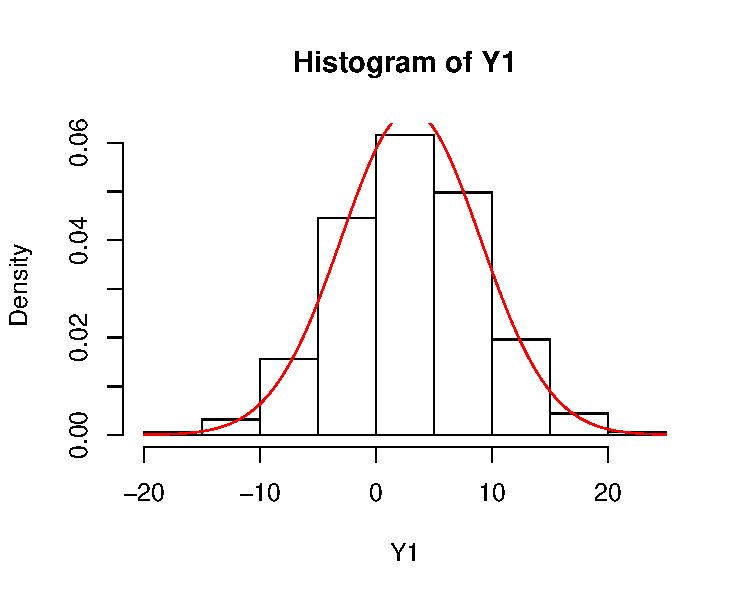
\includegraphics[width=\maxwidth]{figure/ex1_1hist-1} 

}



\end{knitrout}

Next, we create variable $Y_2 = \left( \frac{Y-2}{2} \right)^2$.
$Y_2$ is a quadratic function of $Y$, so we know that distribution of $Y_2$ is not normal. What is more, 
\[\frac{Y-2}{2} \sim N(0,1).\] 
It means that $Y_2$, as a sum of squared standard normally distributed variables, has $\chi^2$ distribution with 1 degree of freedom.

\begin{knitrout}
\definecolor{shadecolor}{rgb}{0.969, 0.969, 0.969}\color{fgcolor}\begin{figure}[H]

{\centering 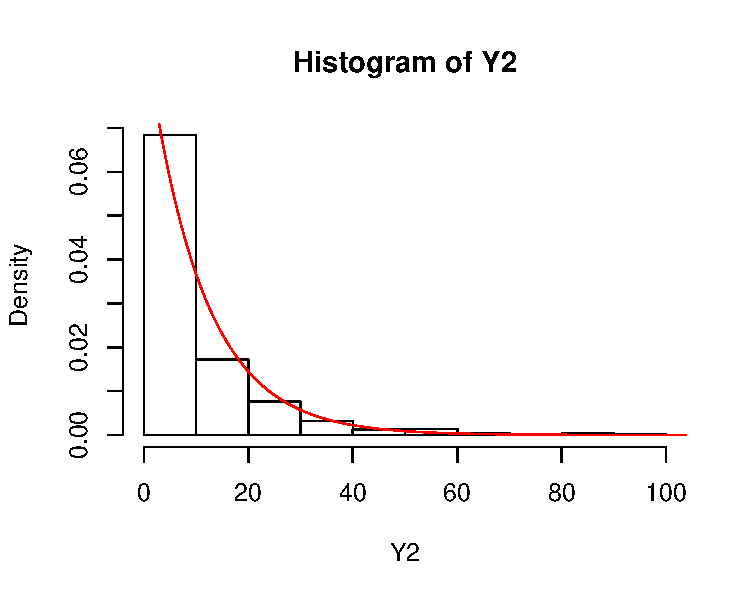
\includegraphics[width=\maxwidth]{figure/ex1_2hist-1} 

}

\caption[Histogram and theoretical probability density function of $Y_2$]{Histogram and theoretical probability density function of $Y_2$}\label{fig:ex1.2hist}
\end{figure}


\end{knitrout}

% EX 1.3

Next we will compute a sequence of means $m_n$ and a sequence of variances $\sigma_n^2$ for the variable~$Y$, where
\[ m_n = \frac{1}{n} \sum_{i=1}^{n} Y_i, \]
\[ \sigma_n = \frac{1}{n} \sum_{i=1}^{n} (Y_i - m_n)^2 \]
and plot the results.

\begin{knitrout}
\definecolor{shadecolor}{rgb}{0.969, 0.969, 0.969}\color{fgcolor}\begin{figure}[H]

{\centering 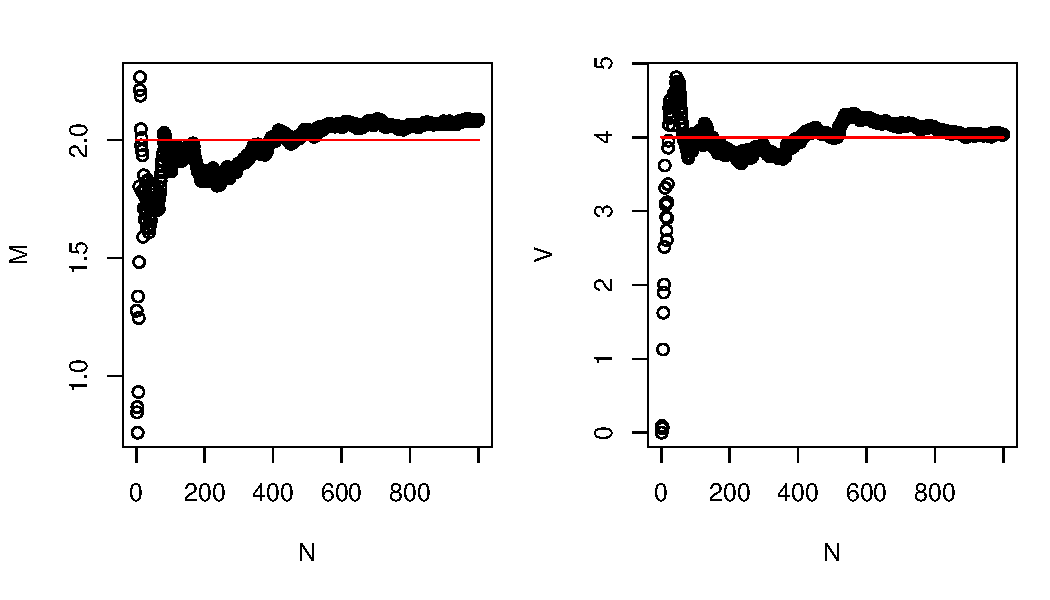
\includegraphics[width=\maxwidth]{figure/ex1_2seq-1} 

}

\caption[Sequence of means and variances and their respective analytical values]{Sequence of means and variances and their respective analytical values.}\label{fig:ex1.2seq}
\end{figure}


\end{knitrout}

The sequences $m_n$ and $\sigma_n^2$ converge to theoretical mean and variance, respectively. To examine the variability of the sequences we can calculate relative errors for both values.

\[ err_{m_n} = \left| \frac{m_n - \mu_n}{\mu_n}  \right| , \qquad
   err_{\sigma_n^2} = \left| \frac{\sigma_n^2 - \sigma_n}{\sigma_n}  \right| \]

\begin{knitrout}
\definecolor{shadecolor}{rgb}{0.969, 0.969, 0.969}\color{fgcolor}\begin{figure}[H]

{\centering 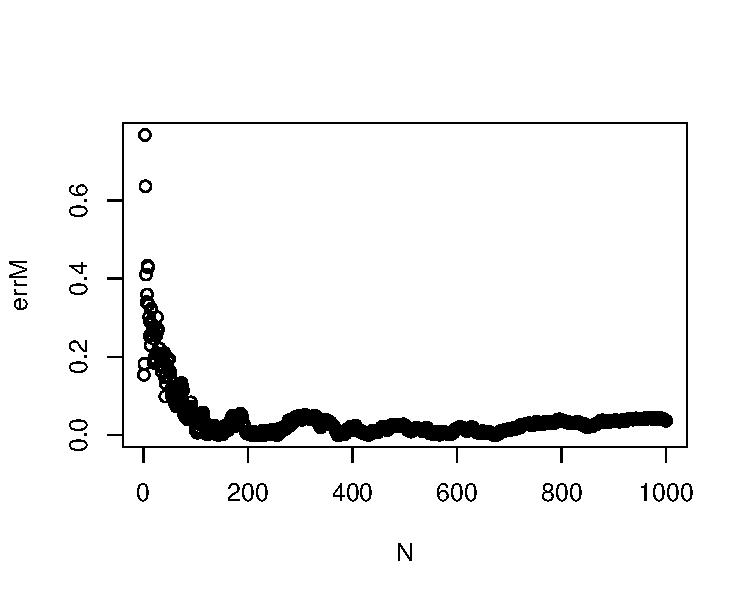
\includegraphics[width=\maxwidth]{figure/ex1_2err-1} 

}

\caption[Relative errors for sequences of means and variances]{Relative errors for sequences of means and variances}\label{fig:ex1.2err}
\end{figure}


\end{knitrout}

For $N>200$ value of the error is less than $10\%$ of theoretical mean.
















%%%%%%%%%%%%%%%%%%%%%%%%%%%%%%%%%%%%%%%%%%%%%%%%%%%%%%%%%%%%%%%%
\section{Exercise 2}

We simulate 10000 times and then plot 2-dimensional random variable $X\sim N(0,I_2)$.

\begin{knitrout}
\definecolor{shadecolor}{rgb}{0.969, 0.969, 0.969}\color{fgcolor}\begin{figure}[H]

{\centering 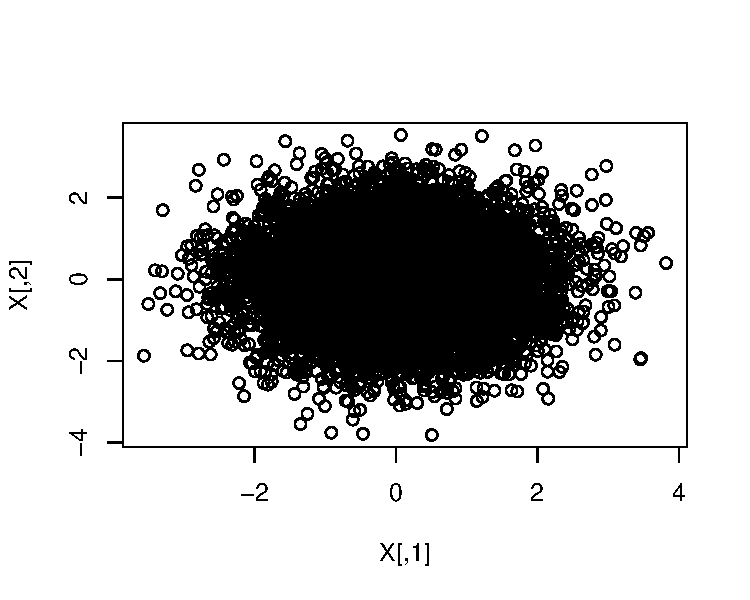
\includegraphics[width=\maxwidth]{figure/ex2X-1} 

}

\caption[2-dimensional random variable $X$ of $N(0,I_2)$ distribution]{2-dimensional random variable $X$ of $N(0,I_2)$ distribution.}\label{fig:ex2X}
\end{figure}


\end{knitrout}

We have to transform variable $X$ into variable $Y \sim N(\mu, \Sigma)$, where 
\[\mu = \left[0,\ 1\right] \quad \text{and }\quad 
  \Sigma = \left[
    \begin{matrix}  
      2   & 0.5 \\
      0.5 & 2
    \end{matrix} 
    \right]
\]
It means that we should find vector $a$ and matrix $A$, such that $Y=A X + a$. 
Expected value of $Y$ is equal to
\[E(Y) = E(AX+a) = A E(X)+a = a, \]
and variance
\[Var(Y) = Var(AX+a) = Var(AX) = A Var(X) A' = A I A' = A A' = \Sigma \]

We know that $\Sigma$ is a symmetric and positive definite matrix, so we can use Cholesky decomposition (chol() function in R) to obtain the value of $A$:
\begin{knitrout}
\definecolor{shadecolor}{rgb}{0.969, 0.969, 0.969}\color{fgcolor}\begin{kframe}
\begin{alltt}
\hlstd{Sigma} \hlkwb{<-} \hlkwd{matrix}\hlstd{(}\hlkwd{c}\hlstd{(}\hlnum{2}\hlstd{,} \hlnum{0.5}\hlstd{,} \hlnum{0.5}\hlstd{,} \hlnum{2}\hlstd{),} \hlnum{2}\hlstd{,} \hlnum{2}\hlstd{)}
\hlkwd{chol}\hlstd{(Sigma)}
\end{alltt}
\begin{verbatim}
##          [,1]      [,2]
## [1,] 1.414214 0.3535534
## [2,] 0.000000 1.3693064
\end{verbatim}
\end{kframe}
\end{knitrout}




\begin{knitrout}
\definecolor{shadecolor}{rgb}{0.969, 0.969, 0.969}\color{fgcolor}\begin{figure}[H]

{\centering 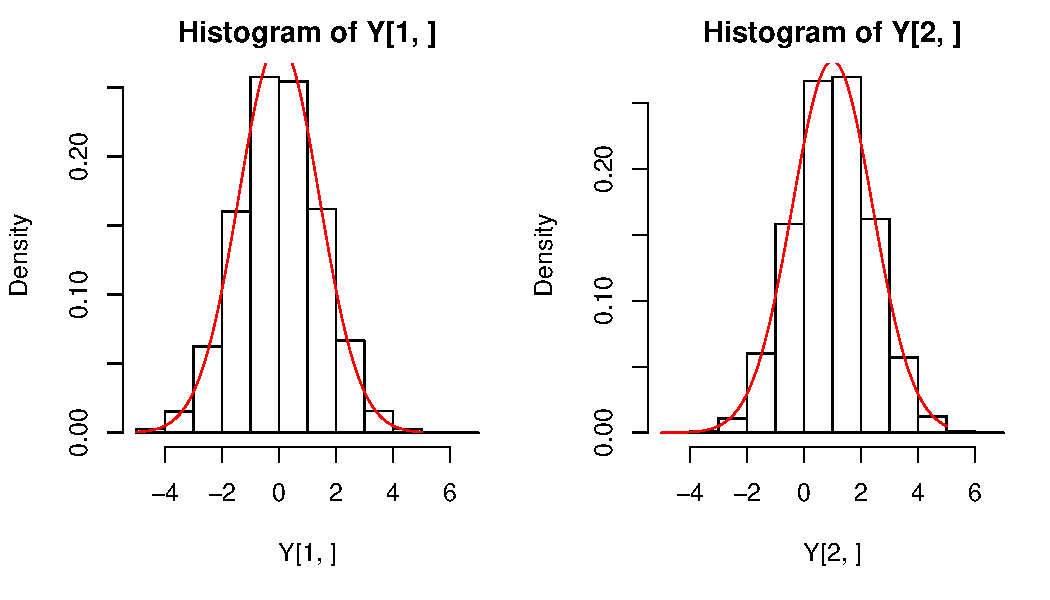
\includegraphics[width=\maxwidth]{figure/ex2checkDistrY2-1} 

}

\caption[Histograms and probability density functions of Y]{Histograms and probability density functions of Y}\label{fig:ex2checkDistrY2}
\end{figure}


\end{knitrout}

Now we can plot the 3D histogram of the random variable $Y = \left[\begin{matrix} 1.414214 & 0.3535534 \\ 0.0 & 1.3693064 \end{matrix} \right]X+\mu$.
\begin{knitrout}
\definecolor{shadecolor}{rgb}{0.969, 0.969, 0.969}\color{fgcolor}\begin{figure}[H]

{\centering 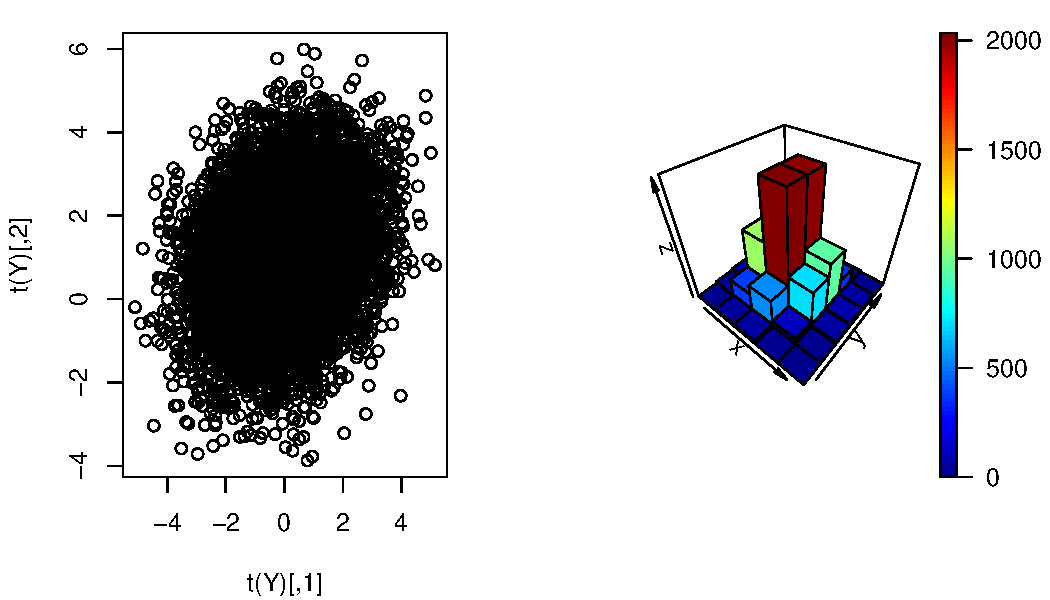
\includegraphics[width=\maxwidth]{figure/ex2_3hist3d-1} 

}

\caption[Random variable $Y$ and its 3D histogram with 30 bins and bars colored according to height]{Random variable $Y$ and its 3D histogram with 30 bins and bars colored according to height.}\label{fig:ex2.3hist3d}
\end{figure}


\end{knitrout}

% exercise 2.4

We are going to transform the variable $Y$ into the variable $Z= (Y-\mu)' \Sigma^{-1} (Y-\mu)$, and $\Sigma$ is a non-singular matrix.
\[
Z = (Y-\mu)' \Sigma^{-1} (Y-\mu) = (Y-\mu)' \Sigma^{-0.5} \Sigma^{-0.5} (Y-\mu) = \left(\Sigma^{-0.5} (Y-\mu)\right)' \left(\Sigma^{-0.5} (Y-\mu)\right)
\]
Let's take $\Sigma^{-0.5} (Y-\mu) = B$. We know that $B \sim N(0,I)$, so $B'B \sim \chi^2(k)$, where $k=2$.


\begin{knitrout}
\definecolor{shadecolor}{rgb}{0.969, 0.969, 0.969}\color{fgcolor}\begin{figure}[H]

{\centering 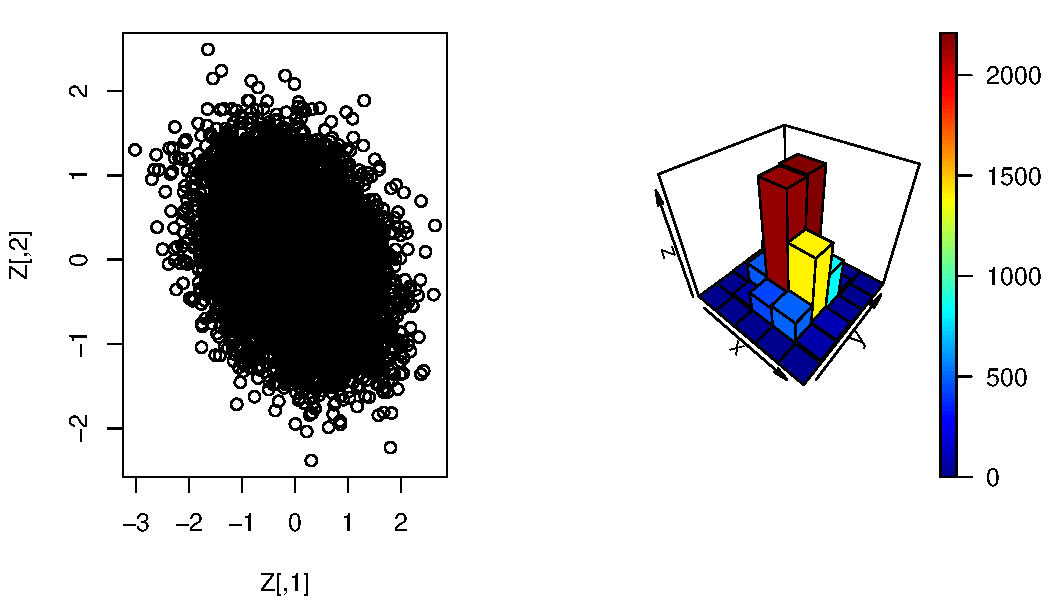
\includegraphics[width=\maxwidth]{figure/ex2_4histZ-1} 

}

\caption[Random variable $Z$ and its 3D histogram with 30 bins and bars colored according to height]{Random variable $Z$ and its 3D histogram with 30 bins and bars colored according to height.}\label{fig:ex2.4histZ}
\end{figure}


\end{knitrout}












%%%%%%%%%%%%%%%%%%%%%%%%%%%%%%%%%%%%%%%%%%%%%%%%%%%%%%%%%%%%%%%%
\section{Exercise 3}


Let $\hat{\beta}$ be a sequence of estimators of a $(K\times 1)$ vector $\beta$, which is asymptotically normal with 
\[ \sqrt{N} (\hat{\beta} - \beta) \rightarrow^d N(0,\Sigma) .\]

% EX 3.1
\subsection{Part 1}

If $R \neq 0$ is an $(M\times K)$ matrix, the asymptotic distribution of $\sqrt{N} (R \hat{\beta} - R \beta) \rightarrow^? N(\mu, \sigma)$. We will compute the mean and the variance of $\sqrt{N} (R \hat{\beta} - R \beta)$.

\[ \mu = E\left(\sqrt{N} (R \hat{\beta} - R \beta) \right) = E\left(\sqrt{N} R( \hat{\beta} - \beta) \right) = R\ E\left(\sqrt{N} ( \hat{\beta} - \beta) \right) = 0 \]
and
\[ \sigma = Var\left(\sqrt{N} (R \hat{\beta} - R \beta)\right) = Var\left(\sqrt{N} R(\hat{\beta} - \beta)\right) 
  =\footnote{From task 2 point 2.}\ R\ Var\left(\sqrt{N} (\hat{\beta} -\beta)\right) R' = R \Sigma R',\]
so 
\[ \sqrt{N} (R \hat{\beta} - R \beta) \rightarrow^d N(0, R \Sigma R'),\ \text{for } R \neq 0. \]


% EX 3.2
\subsection{Part 2}

If $p \lim \hat{A} = A$ then the asymptotic distribution of $\sqrt{N}\hat{A}(\hat{\beta}-\beta) \rightarrow^? N(\mu, \sigma)$. 
We know that if $x_n \rightarrow^d x$ and $p \lim y_n = c$, $x_n y_n \rightarrow^d c x$, so

\[ \sqrt{N}\hat{A}(\hat{\beta}-\beta) \rightarrow^d \sqrt{N} A (\hat{\beta}-\beta) \rightarrow^d N(0, A\Sigma A').  \]


% EX 3.3
\subsection{Part 3}

We will prove that $N \left( \hat\beta-\beta \right)' \hat{\Sigma}^{-1} \left( \hat\beta-\beta \right) \rightarrow^d \chi^2 (K)$ if $\Sigma$ is a non-singular matrix and $p \lim \hat{\Sigma} = \Sigma$.

\begin{gather*}
               \sqrt{N} \left( \hat\beta-\beta \right)' \hat{\Sigma}^{-0.5} \hat{\Sigma}^{-0.5} \left( \hat\beta-\beta \right)\sqrt{N} \\
\downarrow^d \\
               \sqrt{N} \left( \hat\beta-\beta \right)' \Sigma^{-0.5} \Sigma^{-0.5} \left( \hat\beta-\beta \right)\sqrt{N} \\
=           \\
                \left( \sqrt{N} \Sigma^{-0.5} \left( \hat\beta-\beta \right) \right)' \left( \sqrt{N} \Sigma^{-0.5} \left( \hat\beta-\beta \right) \right).
\end{gather*}

Let 
\[C = \left( \sqrt{N} \Sigma^{-0.5} \left( \hat\beta-\beta \right)' \right) \rightarrow\footnote{From task 3 part 1.} N(0, \underbrace{ \Sigma^{-0.5}\Sigma \Sigma^{-0.5} }_{I_K}) \]

We have $C' C$, where $ C \rightarrow^d N(0,\ I_K)$, so 
\[ C' C \rightarrow^d \chi^2 (K). \]


















%%%%%%%%%%%%%%%%%%%%%%%%%%%%%%%%%%%%%%%%%%%%%%%%%%%%%%%%%%%%%%%%

\end{document}
